\documentclass[a4paper,openright,12pt]{article}
\usepackage[utf8]{inputenc}
\usepackage{graphicx}
\usepackage{subfigure}
\usepackage[mathscr]{eucal}
\usepackage{titling}
\usepackage{float}
\usepackage{amsmath}
\usepackage{afterpage}
\usepackage{vmargin}
\usepackage[spanish,es-noshorthands]{babel}
\usepackage{csquotes}
\usepackage{eurosym} 
\usepackage{multirow}
\usepackage{xcolor}
\usepackage[export]{adjustbox}
\usepackage{url}
\usepackage[T1]{fontenc}
\usepackage{inconsolata}
\usepackage{listings}
\usepackage{minted}
\usepackage{amsfonts}
\usepackage[backend=biber, style=authoryear-icomp]{biblatex}
\usepackage[none]{hyphenat}
\sloppy
\usepackage[document]{ragged2e}
\usepackage[shortlabels]{enumitem}
\usepackage{titlesec}
\setcounter{secnumdepth}{4}
\usepackage{datetime}
\usepackage{mfirstuc}
\setlist[enumerate]{itemsep=0mm}
\setlist[itemize]{itemsep=0mm}
\addbibresource{bibliography.bib}

% Packages for FSM
\usepackage{pgf}
\usepackage{tikz}
\usetikzlibrary{arrows,automata}

% Things for Morse
\newcommand{\punto}{\kern+0.3pt\raisebox{0.35ex}{\huge\textbf.}}
\newcommand{\raya}{\kern+0.2pt\raisebox{-0.35ex}{\huge\textbf-}}

% Para generar imágenes mock
\usepackage{duckuments}

\setpapersize{A4}       %  DIN A4
\setmargins{3cm}        % margen izquierdo
{2cm}                   % margen superior
{15cm}                  % anchura del texto
{22.5cm}                % altura del texto
{10pt}                  % altura de los encabezados
{1cm}                   % espacio entre el texto y los encabezados
{0pt}                   % altura del pie de página
{2cm}                   % espacio entre el texto y el pie de página

\begin{document}

\author {Alonso Rodríguez}
\title {Trabajo Tutelado I}

% Título
\maketitle

% Justificamos el texto
\justifying{}

\section{Introducción}
El objetivo de esta práctica es implementar un codificador de código morse mediante el uso de una Máquina de Estado Finito (FSM).
Para simplificar la implementación, trabajaremos sobre un subconjunto de este código, en concreto para los caracteres:
\begin{itemize}
    \item `A' (\punto\raya)
    \item `J' (\punto\raya\raya\raya)
    \item `S' (\punto\punto\punto)
    \item `O' (\raya\raya\raya)
    \item `2' (\punto\punto\raya\raya\raya)
\end{itemize} 

El hardware sobre el que se implementa el sistema se trata de la placa FRDM-KL46Z.

\subsection{Detalles acerca del Código Morse}
\begin{itemize}
    \item La unidad de tiempo no está definida explítamente, así que le llamaremos ``tick''
    \item Los puntos (\punto) duran 1 tick
    \item Las rayas (\raya) duran 3 ticks
    \item El espacio intra-carácter es de 1 tick
    \item El espacio inter-carácter es de 3 ticks
    \item El espacio inter-palabra es de 7 ticks
\end{itemize}


\section{Máquina de Estado Finito}
Siguiendo la notación propuesta en las clases para cada estado, denotamos los estados por: $\frac{\text{nombre}}{\overset{\text{salida}}{\text{delay}}}$

Para la implementación de esta FSM consideramos estados con tres posibles entradas:
\begin{itemize}
    \item Vacío ($\emptyset$): El usuario no pulsa el botón durante más de 1 tick
    \item Punto (\punto): El usuario pulsa el botón durante 1 tick
    \item Raya (\raya): El usuario pulsa el botón durante 3 ticks
\end{itemize}

Asimismo las salidas están denotadas en el formato \texttt{[\text{\textcolor{green}{\punto}}\text{\textcolor{red}{\punto}} `C']}, tal que:
\begin{itemize}
    \item \text{\textcolor{green}{\punto}} para indicar que se enciende el LED verde.
    \item \text{\textcolor{red}{\punto}} para indicar que se enciende el LED rojo.
    \item `C', siendo C uno de los posibles carácteres representables en este subconjunto de morse.
\end{itemize}

La ausencia de salidas se indica con el símbolo $\emptyset$.
\bigskip

El delay se expresa en ticks (\ref{ticklen_duration}) tal que:
\begin{itemize}
    \item lt: indica el tiempo en ticks que debe estar encendido el LED.
    \item dt: indica el tiempo en ticks que deben estar apagados los LEDs.
\end{itemize}
\bigskip

Además, como se detalla en \ref{design_button_translation}, \punto \space significa pulsar SW1, y \raya \space SW2.
\bigskip

Para oxigenar el diagrama, en cada nodo que no se especifica el comportamiento de $\emptyset$, \punto, o \raya, significa que dada esa entrada, se vuelve al estado inicial.

\clearpage

\subsection{Diagrama general de la FSM}
\bigskip\bigskip\bigskip % Dejamos espacio por el pgfinterruptboundingbox que hace que las flechas se nos metan en medio del título de la subsección
\begin{center}
\begin{tikzpicture}[->,>=stealth, shorten >=1pt, auto, node distance=3.2cm, semithick]
    \tikzstyle{every state}=[draw=black,text=black]

    % Nodo inicial
    \node[initial,state] (vacio)                              {$\frac{\text{idle}}{\overset{\emptyset}{\text{lt=1 dt=1}}}$};

    % Camino a A, J
    \node[state]         (1p)     [below right of=vacio]      {$\frac{\punto}{\overset{\text{\textcolor{green}{\punto}}}{\text{lt=1 dt=1}}}$};
    \node[state]         (1p1r)   [below left  of=1p]         {$\frac{\punto\raya}{\overset{\text{\textcolor{green}{\punto}}}{\text{lt=3 dt=1}}}$};
    \node[state]         (1p2r)   [below left  of=1p1r]       {$\frac{\punto\raya\raya}{\overset{\text{\textcolor{green}{\punto}}}{\text{lt=3 dt=1}}}$};
    \node[state]         (1p3r)   [below left  of=1p2r]       {$\frac{\punto\raya\raya\raya}{\overset{\text{\textcolor{green}{\punto}}}{\text{lt=3 dt=1}}}$};

    % Camino a O
    \node[state]         (1r)     [below left  of=vacio]      {$\frac{\raya}{\overset{\text{\textcolor{green}{\punto}}}{\text{lt=3 dt=1}}}$};
    \node[state]         (2r)     [below left  of=1r]         {$\frac{\raya\raya}{\overset{\text{\textcolor{green}{\punto}}}{\text{lt=3 dt=1}}}$};
    \node[state]         (3r)     [below left  of=2r]         {$\frac{\raya\raya\raya}{\overset{\text{\textcolor{green}{\punto}}}{\text{lt=3 dt=1}}}$};

    % Camino a S, 2 desde 1p
    \node[state]         (2p)     [below right of=1p]         {$\frac{\punto\punto}{\overset{\text{\textcolor{green}{\punto}}}{\text{lt=1 dt=1}}}$};
    \node[state]         (3p)     [below right of=2p]         {$\frac{\punto\punto\punto}{\overset{\text{\textcolor{green}{\punto}}}{\text{lt=1 dt=1}}}$};
    \node[state]         (2p1r)   [below left  of=2p]         {$\frac{\punto\punto\raya}{\overset{\text{\textcolor{green}{\punto}}}{\text{lt=3 dt=1}}}$};
    \node[state]         (2p2r)   [below left  of=2p1r]       {$\frac{\punto\punto\raya\raya}{\overset{\text{\textcolor{green}{\punto}}}{\text{lt=3 dt=1}}}$};
    \node[state]         (2p3r)   [below left  of=2p2r]       {$\frac{\punto\punto\raya\raya\raya}{\overset{\text{\textcolor{green}{\punto}}}{\text{lt=3 dt=1}}}$};

    % Puntos finales
    \node[state]         (S)      [below of=3p]               {$\frac{\text{ S }}{\overset{\text{\textcolor{red}{\punto}, `S'}}{\text{lt=3 dt=0}}}$};
    \node[state]         (A)      [below left of=S]           {$\frac{\text{ A }}{\overset{\text{\textcolor{red}{\punto}, `A'}}{\text{lt=3 dt=0}}}$};
    \node[state]         (J)      [below of=1p3r]             {$\frac{\text{ J }}{\overset{\text{\textcolor{red}{\punto}, `J'}}{\text{lt=3 dt=0}}}$};
    \node[state]         (O)      [below of=3r]               {$\frac{\text{ O }}{\overset{\text{\textcolor{red}{\punto}, `O'}}{\text{lt=3 dt=0}}}$};
    \node[state]         (2)      [below of=2p3r]             {$\frac{\text{ 2 }}{\overset{\text{\textcolor{red}{\punto}, `2'}}{\text{lt=3 dt=0}}}$};

    \begin{pgfinterruptboundingbox}
    \path
        (vacio) edge                node {\punto}         (1p)
                edge                node {\raya}          (1r)
                edge [loop above]   node {$\emptyset$}    (vacio)
        (1p)    edge                node {\raya}          (1p1r)
                edge                node {\punto}         (2p)
        (1p1r)  edge                node {\raya}          (1p2r)
                edge [bend right=7] node {$\emptyset$}    (A)
        (1p2r)  edge                node {\raya}          (1p3r)
        (1p3r)  edge                node {$\emptyset$}    (J)
        (2p)    edge                node {\punto}         (3p)
                edge                node {\raya}          (2p1r)
        (3p)    edge                node {$\emptyset$}    (S)
        (2p1r)  edge                node {\raya}          (2p2r)
        (2p2r)  edge                node {\raya}          (2p3r)
        (2p3r)  edge                node {$\emptyset$}    (2)

        (1r)    edge                node {\raya}          (2r)
        (2r)    edge                node {\raya}          (3r)
        (3r)    edge                node {$\emptyset$}    (O)

        % Los de vuelta
        (A)    edge [bend left=240, looseness=1.5,in=250]          node {}                (vacio)
        (J)    edge [bend right=240,looseness=1.5,in=100]         node {}                (vacio)
        (S)    edge [bend left=240, looseness=1,  in=250]          node {}                (vacio)
        (O)    edge [bend right=240,looseness=1,  in=100]         node {}                (vacio)
        (2)    edge [bend right=240,looseness=1.75,  in=100]       node {}                (vacio)
    ;
    \end{pgfinterruptboundingbox}
\end{tikzpicture}
\end{center}


%%%%%%%%%%%%%%%%%%%%%%%%%%%%%%%%%%%%%%%%%%%%%%%%%%%%%%%%%%%%%%%%%%%%%%%%%%%%%%%%%%%%%%%%%%%%%%%%%%%%%%%%%%%%%%%%%%%%%%%%%
%                                                    ESPECIFICACIÓN                                                     %
%%%%%%%%%%%%%%%%%%%%%%%%%%%%%%%%%%%%%%%%%%%%%%%%%%%%%%%%%%%%%%%%%%%%%%%%%%%%%%%%%%%%%%%%%%%%%%%%%%%%%%%%%%%%%%%%%%%%%%%%%
\clearpage
\section{Especificación}
\subsection{Interfaz con el sistema}\label{design_button_translation}
Como se especifica en el enunciado de la práctica, se ha programado el sistema de tal forma que SW1 introduce puntos (\punto) y SW2 rayas (\raya), y el método de lectura se detalla en \ref{reading_method}

\subsection{Flujo del programa}
El flujo del programa consiste en, primeramente la inicialización de todos los parámetros, irq handlers, y variables necesarias, y prosigue con la entrada al bucle infinito que sigue la FSM:
\begin{minted}{c}
    while(1) {
        set_output(state.output)
        delay(state.blinking_time)
        clear_output()
        delay(state.delay_time)
        
        if(...)
            state = state.next_state[...]
        else ...
            state = state.next_state[n]
    }
\end{minted}


%%%%%%%%%%%%%%%%%%%%%%%%%%%%%%%%%%%%%%%%%%%%%%%%%%%%%%%%%%%%%%%%%%%%%%%%%%%%%%%%%%%%%%%%%%%%%%%%%%%%%%%%%%%%%%%%%%%%%%%%%
%                                                    IMPLEMENTACIÓN                                                     %
%%%%%%%%%%%%%%%%%%%%%%%%%%%%%%%%%%%%%%%%%%%%%%%%%%%%%%%%%%%%%%%%%%%%%%%%%%%%%%%%%%%%%%%%%%%%%%%%%%%%%%%%%%%%%%%%%%%%%%%%%
\clearpage
\section{Implementación}
\subsection{Decisiones de diseño}
\subsubsection{Método de lectura}\label{reading_method}
Se ha optado por una lectura de los eventos mediante interrupciones, ya que, a pesar de que el programa no es excesivamente complejo, tampoco pienso que fuese una enorme ventaja el
hacerlo mediante \emph{polling}, que además es posible que nos hiciese tener que lidiar con algunos corner cases extras.

\subsubsection{Timing}\label{ticklen_duration}
Como la duración de cada tick no está explícitamente definida, este se define mediante un parámetro en el código, que por decisión personal
he establecido a 750ms:
\begin{minted}{c}
        #define TICKLEN 750
\end{minted}

Y así multiplicamos la propiedad que guarda cada estado en ticks, por \texttt{TICKLEN}:
\begin{minted}{c}
        msDelay(TICKLEN * fsm_state->led_time);
\end{minted}

\subsubsection{Corner cases}
\begin{enumerate}
    \item Los dos switches se presionan a la vez:
\end{enumerate}
En este caso se ha optado por la opción que permite mayor extensibilidad y es que debido a que la pulsación de cada switch activa una interrupción,
siempre sabremos qué switch se ha pulsado.

Además, debido a la alta velocidad de reloj del microprocesador (en comparación con los tiempos que manejamos los humanos), es altamente improbable que ambos botones coincidan
en el mismo ciclo interno del programa, y por tanto se tratará el botón que por cuestión de microsegundos haya sido pulsado antes.

No se puede forzar esta situación manteniendo pulsados ambos switches, ya que la interrupción solo se activa en el accionado del botón.

De todos modos, si nos fijamos atentamente en el código:

\begin{minted}{c}
    if(sw1){
        fsm_state = fsm_state->next[1];
    }else if(sw2){
        fsm_state = fsm_state->next[2];
    }else{
        fsm_state = fsm_state->next[0];
    }
\end{minted}

Podemos apreciar que en caso de temporizar perfectamente para tener las dos variables a uno, se atendería primero la del switch 1, deshaciendo ese posible comportamiento
indeseado o no definido, y permitiendo (a pesar de que sería necesario añadir unos márgenes para poder realizarlo consistentemente) realizar alguna acción especial al pulsar ambos
botones simultáneamente.

\subsection{Detalles de Implementación}
\subsubsection{Estado}
\begin{minted}{c}
typedef const struct _state {
    const uint8_t output;      // Estructura bit-wise: tzyx dcba
                               //    a: LED verde (1=on, 0=off)
                               //    b: LED rojo encendido ('')
                               // Así, si queremos encender el led verde y
                               //  el rojo será 0000 0011.
                               // Pero haciendo uso de los #define superiores,
                               //  podremos escribir LED_GREEN | LED_RED 

    const uint8_t led_time;    // Tiempo en ticks. Este valor será multiplicado
                               //  por TICKLEN ms (definido arriba)

    const uint8_t delay_time;  // Idem pero para el retardo despues del encendido
                               //  del LED
    
    const char character;      // Carácter que se mostrará en el LCD. 0 indica
                               //  ausencia de carácter
    
    /* {no_input, dot, line} */
    const struct _state *next[3];
} state;
\end{minted}

Por si el código no fuese lo suficientemente autodescriptivo, contamos con cuatro constantes dentro de cada estado, que nos definen los valores de:
\begin{itemize}
    \item \texttt{output} - 8 bits que nos indican si se debe encender el led verde o rojo.
    \item \texttt{led\_time} - Nos indica el tiempo en tick que debe permanecer encendido el LED.
    \item \texttt{delay\_time} - Nos indica el tiempo que debe permanecer el LED apagado.
    \item \texttt{character} - Es un char (tambien un entero de 8 bits al fin y al cabo) que indica la salida por LCD.
    \item \texttt{*next[]} - Almacena las referencias a los siguientes estados, en concreto: \begin{enumerate}
        \item \texttt{no\_input [0]}: Apunta al estado al que se transiciona en caso de no recibir input antes de \texttt{delay\_time}.
        \item \texttt{dot [1]}: Apunta al estado al que se transiciona en caso de recibir un punto antes de \texttt{delay\_time}.
        \item \texttt{line [2]}: Apunta al estado al que se transiciona en caso de recibir una raya antes de \texttt{delay\_time}.
    \end{enumerate}
\end{itemize}


\subsubsection{Máquina de estados}
Se ha implementado la máquina de estado finito como un array de estados, y como se indica en las transparencias de teoría, se ha establecido un `alias' a cada estado
mediante \texttt{\#defines}, tal que:
\begin{minted}{c}
    #define s0        &fsm[0]
    // [...]
    #define s1r       &fsm[1]
    // [...]
    #define fsO       &fsm[13]

    #define LED_GREEN 0x1
    #define LED_RED   0x1<<1

    state fsm[] = {
        {0, 0, 0, 0, {s0, s1p, s1r}},               // s0
        // [...]
        {LED_GREEN, 3, 1, 0, {s0, s0, s2r}},        // s1r
        // [...]
        {LED_RED, 3, 0, 'O', {s0, s0, s0}},         // fsO
    };
\end{minted}


%%%%%%%%%%%%%%%%%%%%%%%%%%%%%%%%%%%%%%%%%%%%%%%%%%%%%%%%%%%%%%%%%%%%%%%%%%%%%%%%%%%%%%%%%%%%%%%%%%%%%%%%%%%%%%%%%%%%%%%%%
%                                                          LCD                                                          %
%%%%%%%%%%%%%%%%%%%%%%%%%%%%%%%%%%%%%%%%%%%%%%%%%%%%%%%%%%%%%%%%%%%%%%%%%%%%%%%%%%%%%%%%%%%%%%%%%%%%%%%%%%%%%%%%%%%%%%%%%
\clearpage
\section{Comportamiento del LCD}
En el programa de ejemplo `StopWatch' que se nos provee, podemos observar la forma en la que se maneja el LCD de nuestra placa:

\subsection{Inicialización}
Para esto contamos con `slcdInitialize'.

Para inicializarlo, tenemos que habilitarle la señal de reloj para los puertos B, C, D, E, y al propio módulo sLCD.

Tras ello configuramos los pines, y configuramos el registro del sLCD \texttt{(LCD->GCR)}.

Posteriormente continuamos configurando más parámetros, que no voy a tratar uno por uno, pero que con ellos sacamos en conclusión que el LCD es un periférico más, que por
supuesto es más complejo de usar que un único LED, pero que al final del día, tiene un funcionamiento similar, es decir, tenemos que activarle señales de reloj, configurar
sus pines y su(s) registro(s), etc.

\subsection{Impresión de Caracteres}
La función más interesante (y que probablemente más vamos a usar) en slcd.c es `slcdSet', puesto que es la que hace el trabajo por nosotros de qué mostrar en que sitio,
que número, y lo hace de forma muy sencilla.

Para los que estamos acostumbrados a programar sistemas como Arduino o similares, es un comportamiento muy parecido: En Arduino escribíamos directamente el número en binario,
como por ejemplo 0b01111111 para el número 8. Aquí tenemos unos \#define, cada uno activando un bit.

Así, podemos hacer las cosas un poco más ``elegantes'' usando bitwise-or. Por ejemplo, el 8 sería:

\begin{minted}{c}
LCD->WF8B[LCD_Front_Pin[((2*digit)-2)]] = (LCD_S_G | LCD_S_E |
                                           LCD_S_D | LCD_S_F);
LCD->WF8B[LCD_Front_Pin[((2*digit)-1)]] = (LCD_S_A | LCD_S_B | LCD_S_C);
\end{minted}
donde hacemos un or de cada uno de los bits que encienden un segmento.

\subsubsection{Detalles del panel LCD}
Además, el módulo sLCD con el que contamos tiene una particularidad, y es que cada dígito está dividido en dos subsegmentos, FP0 y FP1, tal que

\begin{samepage}
\begin{verbatim}
        FP0 - Front Plane 0             FP1 - Front Plane 1
        f |_g                           a_
        e |_                              | b
            d                           c |. dot
\end{verbatim}
\end{samepage}
por lo que tenemos que poner los flags en el sitio correcto, \texttt{((2*digit)-2)} para FP0, y \texttt{((2*digit)-1)} para FP1.

Esta forma de acceder a los segmentos nos indica que estamos ante un LCD con dígitos multiplexados en dos vías, la primera siendo el FP0, y la segunda FP1. \autocite[430]{zhu2018embedded}

Es decir, que los sectores (d,e,f,g) $\in$ FP0 están conectados a una misma tierra, así como (a,b,c,dot) $\in$ FP1. Podemos concluir por esto que contamos con
un \emph{Duty Ratio} de $\frac{1}{2}$.

Sabiendo esto, si realizamos ingeniería inversa a \texttt{slcd.h}, podemos ver lo siguiente:
\begin{minted}{c}
#define LCD_S_D 0x11
#define LCD_S_E 0x22
#define LCD_S_G 0x44
#define LCD_S_F 0x88

#define LCD_S_DEC 0x11
#define LCD_S_C 0x22
#define LCD_S_B 0x44
#define LCD_S_A 0x88
\end{minted}

Y podemos dibujar el circuito que implementa el LCD de nuestra placa, en el que (d,dec), (e,c), (g,b), (f,a) son los segmentos que están conectados a las líneas de
tensión que nosotros activamos o desactivamos desde el control del programa.
\begin{center}
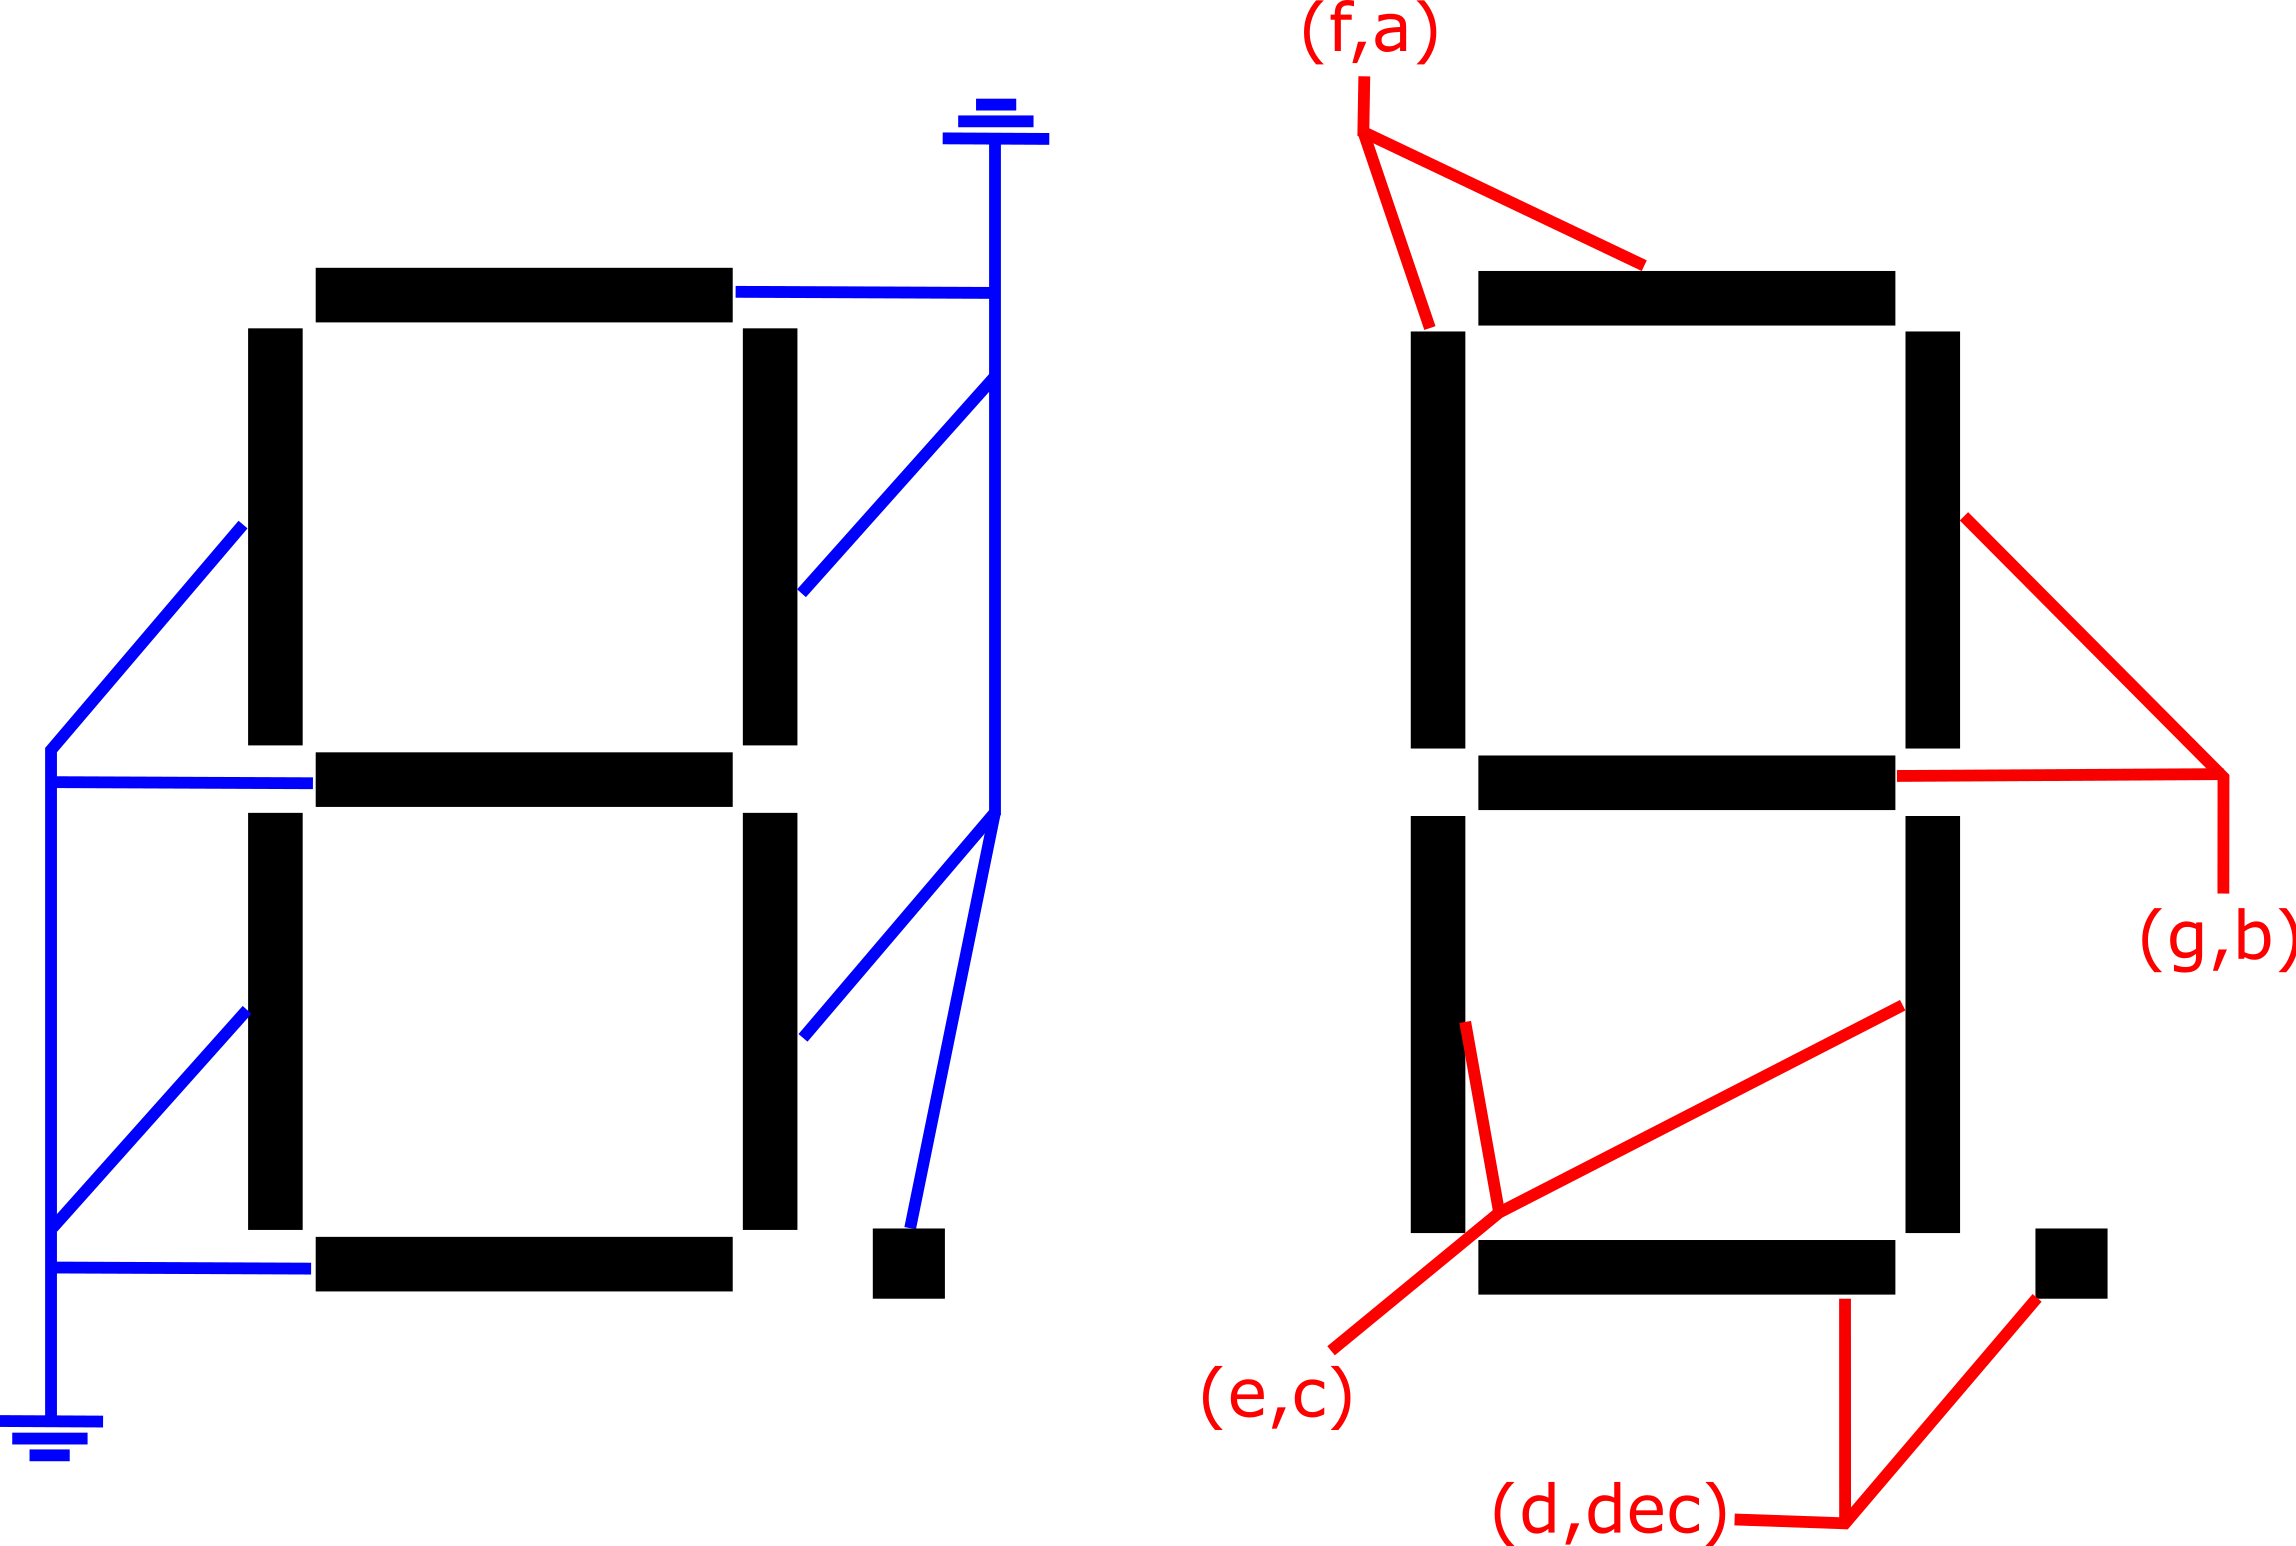
\includegraphics[scale=0.5]{img/digits.png}
\end{center}

\subsection{Funciones}
Contamos con tres funciones autodescriptivas, que son:
\begin{enumerate}[a]
    \item slcdDisplay   \label{otras_func_slcdDisplay}
    \item slcdClear     \label{otras_func_slcdClear}
    \item slcdDemo      \label{otras_func_slcdDemo}
\end{enumerate}


`slcdDisplay' (\ref{otras_func_slcdDisplay}), nos muestra el número de 16 bits `value' en el formato deseado (esto segundo aún no está implementado).

`slcdClear' (\ref{otras_func_slcdClear}), que hace lo que su nombre indica, borrar el display.

`slcdDemo' (\ref{otras_func_slcdDemo}), que es el que se ejecuta en el programa StopWatch, y que muestra cada uno de los números en hexadecimal en la pantalla uno
despues de otro, de forma circular, limpiando la pantalla tras escribir cada uno de ellos.

Se ve muy claramente en el código:
\begin{minted}{c}
    for(i=0; i < 0x10; i++){
        slcdClear();
        slcdSet(i, i%4 + 1);
        msDelay(300);
        slcdClear();
    }   
\end{minted}

También he tenido que corregir el código de `slcdSet', y `slcdErr', ya que los números 1, 2 y 3 no estaban programados,
y 0xB estaba con las regiones del dígito intercambiadas, y falta por implementar una parte de `slcdDisplay', que no es necesario completar ya que no se usa.

\subsection{Funciones nuevas}
Se ha implementado una nueva función que muestra los caracteres alfanuméricos en el LCD:
\begin{minted}{c}
    void slcdSetChar(char c, uint8_t digit)
\end{minted}

Donde \texttt{digit} es la posición de izquierda a derecha [1..4] en el LCD del carácter a imprimir, y que soporta como entradas para \texttt{c}:
\begin{itemize}
    \item `O'
    \item `2'
    \item `S'
    \item `J'
    \item `A'
\end{itemize}



\printbibliography[]{}
\end{document}